\section{Experiments and Results}
\label{sec:experiments}

\subsection{Setup}
All experiments ran on a single laptop GPU (NVIDIA GeForce RTX 3070 Ti, 8\,GB) with Python 3.12, PyTorch 2.5.1 (CUDA 12.1) and the Hugging Face \texttt{transformers} library 4.57. The architectures, optimizers and hyperparameters are described in Section~\ref{sec:design}. Table~\ref{tab:setup} summarizes the training configuration. All numbers in this section come from just \emph{one} random seed (seed 0) per setting, so they are preliminary; the proposal's three-seed protocol is part of the remaining work.

\begin{table}[t]
\caption{Training configuration.}
\label{tab:setup}
\centering
\small
\begin{tabular}{lll}
\toprule
 & TextCNN & DistilBERT \\
\midrule
Input embeddings & GloVe 300d, frozen & pretrained, fine-tuned \\
Max.\ length & 256 tokens & 256 word pieces \\
Optimizer & AdamW & AdamW \\
Learning rate & $10^{-3}$ & $3\times10^{-5}$ \\
Batch size & 64 & 32 \\
Epochs & 6 & 2 \\
Training reviews & 314{,}504 (all) & 100{,}000 (random subset) \\
Precision & fp32 & fp16 mixed \\
Loss settings & \multicolumn{2}{c}{$\alpha=1$, $\lambda=0.5$ (not tuned)} \\
Model selection & \multicolumn{2}{c}{best validation Macro F1} \\
\bottomrule
\end{tabular}
\end{table}

\subsection{Dataset Statistics}
Table~\ref{tab:splits} lists the split sizes. The three splits have almost the same rating distribution (Fig.~\ref{fig:rating}), so the split by product does not introduce a distribution shift. The data is strongly imbalanced: about 64\% of reviews have 5 stars, while 2-star reviews make up only about 5\%. A classifier that always predicts 5 gets roughly 64\% accuracy, so accuracy alone is misleading. This is why we also use Macro F1 and the distance-based metrics (MAE, large error rate). Reviews are short: the median length is 57 words in the training set (mean 79.5), and the 95th percentile is 214 words (Fig.~\ref{fig:length}). A maximum sequence length of 256 tokens holds the full review for 96.0\% of reviews with the TextCNN tokenizer and 94.2\% with the DistilBERT tokenizer (Section~\ref{sec:design}).

\begin{table}[t]
\caption{Dataset split statistics after cleaning (393{,}135 reviews in total).}
\label{tab:splits}
\centering
\begin{tabular}{lrr}
\toprule
Split & Reviews & Products \\
\midrule
Train & 314,504 & 54,104 \\
Val & 39,171 & 6,428 \\
Test & 39,460 & 6,962 \\
\bottomrule
\end{tabular}

\end{table}

\begin{figure}[t]
\centering
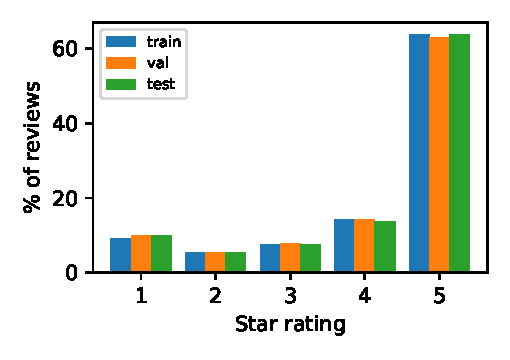
\includegraphics[width=\columnwidth]{rating_distribution.pdf}
\caption{Rating distribution in each split.}
\label{fig:rating}
\end{figure}

\begin{figure}[t]
\centering
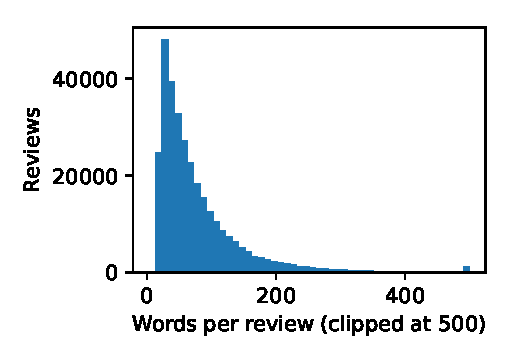
\includegraphics[width=\columnwidth]{review_length.pdf}
\caption{Review length in words (training set, clipped at 500).}
\label{fig:length}
\end{figure}

\subsection{Pilot Experiments}
Before the main runs we measured training time and memory on subsets. TextCNN is cheap: one epoch over the full training set takes about 45--70 seconds and the peak GPU memory is 0.23\,GB. DistilBERT is much more expensive. Fine-tuning on 20{,}000 reviews for one epoch took 155 seconds with every review padded to 256 word pieces, and 102 seconds with dynamic padding (a reduction of about one third), at a peak GPU memory of 2.7\,GB. Extrapolated from this pilot, one epoch over the full training set would take about 27 minutes. We therefore chose to train DistilBERT on a 100{,}000-review subset for two epochs in this report. In practice, an epoch on this subset took 20 to 30 minutes, much longer than the roughly 9 minutes the extrapolation suggested. Part of the gap is the evaluation on the full validation set after every epoch; we did not look into the rest. With the measured speed, a full epoch would take an hour or more, and three losses with three seeds and two epochs on the full training set would take more than 20 hours, so the subsample is needed to finish in the time we have.

\subsection{Main Results}
Table~\ref{tab:main} lists the test results of all six settings. The test set was used once per run, with the checkpoint that had the best validation Macro F1.

\begin{table*}[t]
\caption{Test results (seed 0; mean $\pm$ std once several seeds are available). Lower is better for MAE and large error rate; higher is better for accuracy and Macro F1. Train time is in minutes.}
\label{tab:main}
\centering
\begin{tabular}{llcccccc}
\toprule
Model & Loss & Seeds & Accuracy & Macro F1 & MAE & Large Err. & Train (min) \\
\midrule
\multirow{3}{*}{TextCNN} & CE & 1 & 0.747 & 0.495 & 0.395 & 0.085 & 5.4 \\
 & OLL & 1 & 0.733 & 0.508 & 0.373 & 0.070 & 7.0 \\
 & MLL & 1 & 0.744 & 0.509 & 0.378 & 0.076 & 8.2 \\
\midrule
\multirow{3}{*}{DistilBERT} & CE & 1 & 0.767 & 0.575 & 0.311 & 0.051 & 51.7 \\
 & OLL & 1 & 0.746 & 0.556 & 0.320 & 0.048 & 43.3 \\
 & MLL & 1 & 0.760 & 0.574 & 0.317 & 0.052 & 39.3 \\
\bottomrule
\end{tabular}

\end{table*}

\paragraph{TextCNN.} Both ordinal losses reduce the distance-based errors compared with cross entropy. OLL lowers the MAE from 0.395 to 0.373 and the large error rate from 8.5\% to 7.0\%, and MLL gives 0.378 and 7.6\%. Macro F1 does not drop; it rises slightly from 0.495 to 0.508 (OLL) and 0.509 (MLL). The price is a lower accuracy for OLL (74.7\% to 73.3\%), while MLL stays close to cross entropy (74.4\%). OLL and MLL also trained somewhat more slowly than cross entropy in our runs (Table~\ref{tab:main}); we have not checked whether this comes from the loss itself or just from how busy the GPU was.

\paragraph{DistilBERT.} Here the ordinal losses do not help on the main distance metric. Cross entropy gives MAE 0.311 and a large error rate of 5.1\%. OLL raises the MAE to 0.320 (+2.8\%) and lowers the large error rate only to 4.8\% ($-6.7\%$), while Macro F1 falls from 0.575 to 0.556 and accuracy from 76.7\% to 74.6\%. MLL is close to cross entropy on all metrics (MAE 0.317, large error rate 5.2\%, Macro F1 0.574, accuracy 76.0\%). The OLL run reached its best validation Macro F1 after the first epoch, whereas the other two runs did so after the second. The differences between the three losses are small, and with only one seed we cannot tell which of them are real. Train times in Table~\ref{tab:main} should not be compared between losses, because the GPU was shared with other work to different degrees during the runs.

\paragraph{Architectures.} DistilBERT is clearly stronger than TextCNN with every loss, even though it saw only 100{,}000 training reviews for two epochs, against 314{,}504 reviews for six epochs for TextCNN. With cross entropy its Macro F1 is 0.575 against 0.495, its MAE 0.311 against 0.395, and its large error rate 5.1\% against 8.5\%. The benefit of an ordinal loss is also smaller for the stronger model: the large error rate of TextCNN falls by 17.4\% with OLL, whereas that of DistilBERT falls by 6.7\%, and the MAE does not improve at all. One possible reason is that DistilBERT already makes few large errors with cross entropy, so there is less to gain, but our data cannot confirm this.

\subsection{Reference Baselines}
\label{sec:baselines}
To put the neural results in context, we also trained three simple non-neural references on the same splits: a majority predictor (always 5 stars) and a linear classifier on TF-IDF features of word unigrams and bigrams (at most 60{,}000 features, minimum document frequency 3, sublinear term frequency), trained with stochastic gradient descent on a logistic loss. The linear classifier was fitted once without class weights and once with class weights inversely proportional to the training class frequencies. The settings were fixed in advance and not tuned; three seeds were run, and their standard deviations are about 0.001 or less on all metrics. Table~\ref{tab:baselines} lists the test results.

\begin{table}[t]
\caption{Test results of the non-neural reference baselines (TF-IDF: mean of three seeds).}
\label{tab:baselines}
\centering
\begin{tabular}{lcccc}
\toprule
Baseline & Accuracy & Macro F1 & MAE & Large Err. \\
\midrule
Majority (always 5 stars) & 0.636 & 0.156 & 0.839 & 0.226 \\
TF-IDF, unweighted & 0.733 & 0.450 & 0.456 & 0.104 \\
TF-IDF, class-balanced & 0.729 & 0.528 & 0.408 & 0.081 \\
\bottomrule
\end{tabular}

\end{table}

Two things matter for reading the main results. First, the majority predictor reaches 63.6\% accuracy but a Macro F1 of only 0.156, which confirms that accuracy alone is misleading on this data. Second, class weights alone change the distance-based errors quite a bit: compared with the unweighted linear model, the weighted one lowers the MAE from 0.456 to 0.408 ($-10.4\%$) and the large error rate from 10.4\% to 8.1\% ($-22\%$), and raises Macro F1 from 0.450 to 0.528, with no ordinal information at all. These gains are at least as large as those of OLL and MLL over unweighted cross entropy for TextCNN (Table~\ref{tab:main}). The linear model with class weights is also close to TextCNN with cross entropy (MAE 0.408 against 0.395, large error rate 8.1\% against 8.5\%) and has a higher Macro F1 (0.528 against 0.495). Part of the benefit of the ordinal losses for TextCNN may therefore come from reducing the bias towards the majority class and not from their use of the rating order. We have not yet run cross entropy with class weights on the neural models, which is the control we need to separate the two effects, so it is on our list of remaining work. DistilBERT is clearly better than all three baselines.

\subsection{Error Analysis}
\label{sec:errors}
Figure~\ref{fig:confusion_textcnn} shows row-normalized confusion matrices of the TextCNN models. With cross entropy, the model strongly favors the majority class: 76\% of all test reviews are predicted as 5 stars, although only about 64\% are 5-star reviews. It sends 72\% of the true 4-star reviews, 34\% of the 3-star reviews and 13\% of the 1-star reviews to 5 stars. At the other end, 41\% of the true 2-star reviews are predicted as 1 star, and only 20\% are recognized correctly.

OLL changes this pattern the way it is supposed to. It predicts 5 stars less often (71\% of all reviews), and the large confusions drop: 1-star reviews predicted as 5 stars fall from 13\% to 7\%, and 3-star reviews predicted as 5 stars from 34\% to 20\%. The mistakes move to neighboring ratings instead; for example, the recall of the 2-star class rises from 20\% to 39\% and that of the 4-star class from 14\% to 23\%. This comes at a cost for the extreme classes, whose recall falls (1 star: 77\% to 62\%; 5 stars: 97\% to 93\%), which explains the lower accuracy of OLL. MLL lies between the two, with a pattern closer to cross entropy for the 4-star and 5-star classes.

Figure~\ref{fig:error_distance_textcnn} shows the same trend as the share of test reviews that are off by 0 to 4 stars. Compared with cross entropy, OLL has more errors of exactly one star (19.7\% vs.\ 16.8\%) but fewer errors of three stars (1.4\% vs.\ 1.6\%) and four stars (1.1\% vs.\ 2.1\%). This is the trade-off an ordinal loss is meant to make: it accepts more small errors to get fewer large ones.

\begin{figure*}[t]
\centering
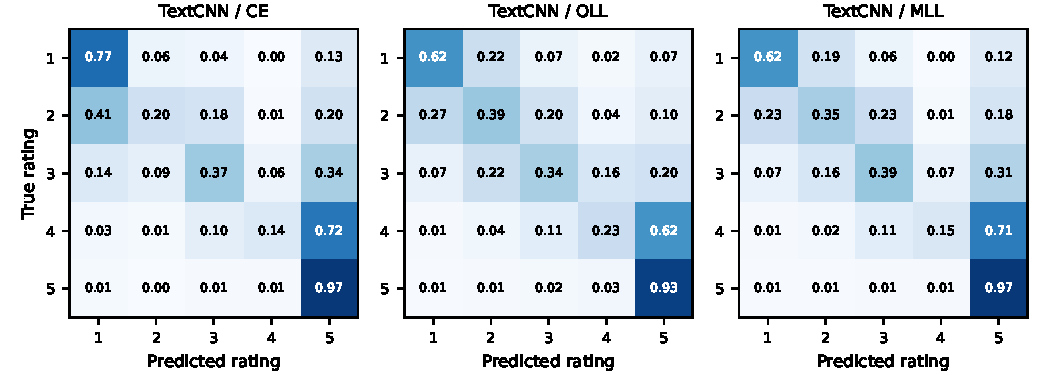
\includegraphics[width=\textwidth]{confusion_textcnn.pdf}
\caption{Row-normalized confusion matrices of the TextCNN models on the test set (rows: true rating, columns: predicted rating).}
\label{fig:confusion_textcnn}
\end{figure*}

\begin{figure}[t]
\centering
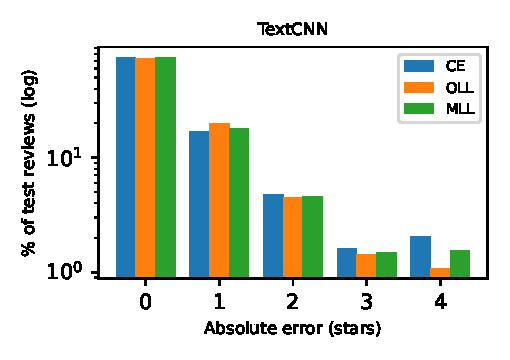
\includegraphics[width=\columnwidth]{error_distance_textcnn.pdf}
\caption{Share of test reviews by absolute error (in stars) for the TextCNN models; the vertical axis is logarithmic.}
\label{fig:error_distance_textcnn}
\end{figure}

\paragraph{Examples.} Table~\ref{tab:examples} shows test reviews on which the TextCNN models behave differently. Among the reviews we inspected in which cross entropy is wrong by three or more stars, several mix positive and negative statements and are pushed into the majority class; the first four rows are of this kind, and OLL (and, in some cases, MLL) predicts a closer rating. Among all 39{,}460 test reviews, 361 are predicted by cross entropy with an error of at least three stars but by OLL within one star, whereas the reverse (OLL off by at least three stars while cross entropy is within one star) happens for 158 reviews. The last two rows are examples of the second case, where OLL fails on reviews that are positive overall. So the gain of OLL on large errors is a net effect, not an improvement everywhere.

\begin{table*}[t]
\caption{Test reviews with different TextCNN predictions (T: true rating; CE, OLL, MLL: predicted rating). Review texts are shown in full.}
\label{tab:examples}
\centering
\small
\begin{tabular}{p{11.5cm}cccc}
\toprule
Review & T & CE & OLL & MLL \\
\midrule
Love the flavor of this gum but the flavor just doesn't last and the gum gets tough quickly. & 2 & 5 & 3 & 5 \\
Seemed like a great idea at first, but these hearts where mushy (overcooked) not good in salads, best in caserole or cooked dished. & 2 & 5 & 3 & 3 \\
They taste good but they'll send you to the toilet quickly and burn you up. There's better beef jerky out there. & 3 & 5 & 4 & 3 \\
The gum is tart and sweet for the initial chew but the flavor is almost gone in ten minutes. & 3 & 5 & 3 & 5 \\
\midrule
We were recommended to use this formula due to severe food allergies to my 5 month old son. His spit-ups stopped after using this and stools also became better. & 5 & 5 & 2 & 5 \\
Hello, The slim jims came in a timely manner, as soon as I expected. Most of them were good, however, I found one of them that was uneatable. & 4 & 3 & 1 & 2 \\
\bottomrule
\end{tabular}
\end{table*}

\paragraph{DistilBERT.} Figures~\ref{fig:confusion_distilbert} and~\ref{fig:error_distance_distilbert} show the same analysis for DistilBERT. The cross-entropy model predicts 5 stars for 67.5\% of the test reviews (64\% are 5-star), much less than TextCNN (76\%). OLL reduces this share to 64.3\% and raises the recall of the 4-star class from 29\% to 42\%, but lowers the recall of 1-star (79\% to 68\%), 2-star (35\% to 29\%) and 3-star (53\% to 47\%) reviews. It has the most one-star errors (20.6\% against 18.2\%) and the fewest errors of four stars (0.4\% against 1.0\%). MLL again lies close to cross entropy.

\begin{figure*}[t]
\centering
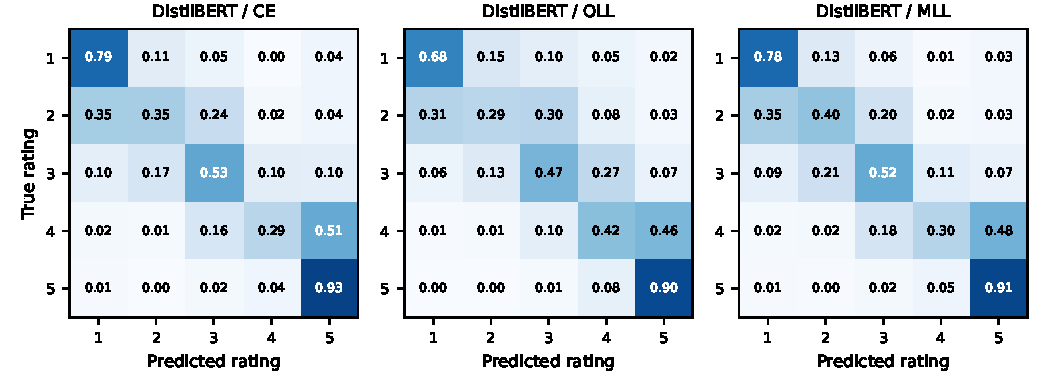
\includegraphics[width=\textwidth]{confusion_distilbert.pdf}
\caption{Row-normalized confusion matrices of the DistilBERT models on the test set.}
\label{fig:confusion_distilbert}
\end{figure*}

\begin{figure}[t]
\centering
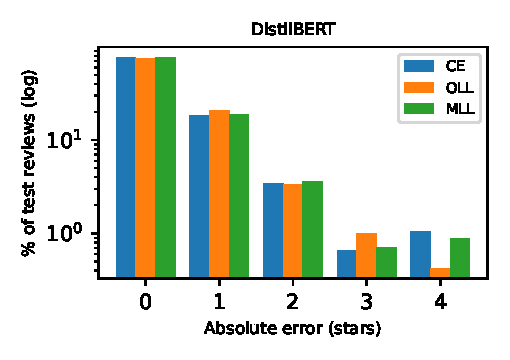
\includegraphics[width=\columnwidth]{error_distance_distilbert.pdf}
\caption{Share of test reviews by absolute error (in stars) for the DistilBERT models; the vertical axis is logarithmic.}
\label{fig:error_distance_distilbert}
\end{figure}

\subsection{Success Criteria Check}
We now check the three conditions from Section~\ref{sec:criteria} against cross entropy. For TextCNN, OLL reduces MAE by 5.4\% and the large error rate by 17.4\% while Macro F1 changes by $+0.013$; MLL reduces MAE by 4.4\% and the large error rate by 10.3\% with a Macro F1 change of $+0.014$. Both therefore meet all three conditions for TextCNN, but only relative to unweighted cross entropy: Section~\ref{sec:baselines} shows that class weights alone can give gains of similar size, so the result may partly reflect the correction of the majority-class bias. This is a single-seed result, so we cannot say yet how much of the difference is just random variation. For DistilBERT, OLL increases the MAE by 2.8\%, reduces the large error rate by 6.7\% and lowers Macro F1 by 0.018, so it meets only the large-error condition and fails the other two. MLL increases the MAE by 1.9\% and the large error rate by 2.3\%, with a Macro F1 change of $-0.0006$; it meets only the Macro F1 condition. The hypothesis is therefore supported for TextCNN but not for DistilBERT in this first run. We will repeat the check with three-seed averages.

\subsection{Cross-Category Evaluation (Optional)}
Not carried out so far; see Section~\ref{sec:conclusion}.
